\section{Introduction}

\subsection{Motivation}

Storage plays an important role in \ac{HPC} environments, with demands on storage infrastructure increasing steadily as modern workloads continue to grow. In addition to capacity, fast and low-latency access to data ensure that compute nodes can spend more time on computation tasks rather than waiting for data, increasing compute efficiency. Given that \ac{HPC} clusters' resources are often shared among multiple users, file systems should also be able to handle requests from multiple users with an acceptable level of performance.

Incumbents in the \ac{HPC} space, such as Lustre, are designed specifically to be \ac{HPC} file systems~\cite{lustre-homepage}. This allows for the design of the file system to be highly optimized for these use cases, with a proven track record and market share over time. However, this highly optimized nature presents issues in terms of hardware complexity and cost, as well as maintainability, due to the rigid requirements of these file systems.

Ceph emerges from this background as a potentially compelling alternative to incumbent file systems due to its flexible design. It is a fully software-defined, distributed storage system, designed to be a ``catch-all'' solution---with the express intent of being deployable on commodity hardware, while maintaining flexibility for larger deployments. However, Ceph has not yet seen wide deployment in the \ac{HPC} space, with \acs{HPC}-specific file systems still making up the majority of the backing storage for supercomputers in the IO500 rankings for storage performance~\cite{io500-full-list}, as shown in \Cref{fig:io500-storage-share}.

\begin{figure}[H]
    \centering
    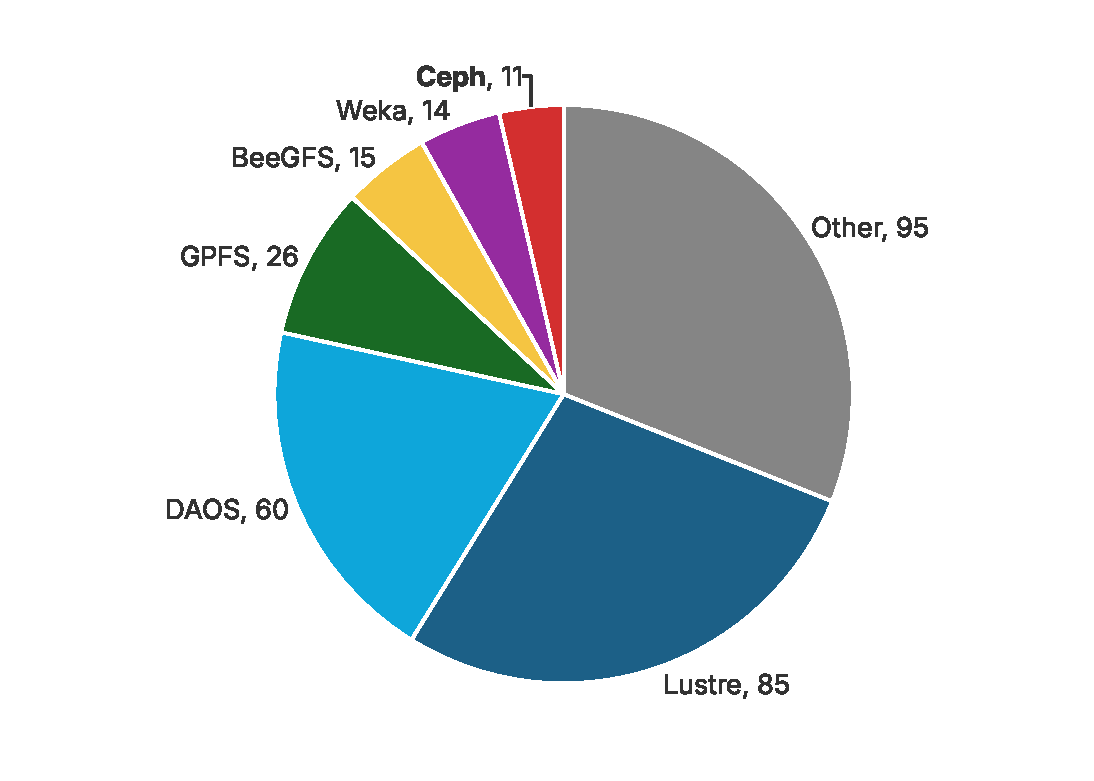
\includegraphics[height=9cm]{assets/charts/storage_market_share.pdf}
    \caption[File System Share of IO500 Results]{The share of file systems used in the IO500 rankings for storage performance~\cite{io500-full-list}}
    \label{fig:io500-storage-share}
\end{figure}

While the IO500 rankings are far from a benchmark of every \ac{HPC} system in existence, it still roughly demonstrates that file systems designed specifically for \ac{HPC} make up the majority of file systems used. Additionally, Ceph did not reach the top 100 of all historical IO500 rankings, although it did achieve 42nd place in the production-grade node list as of March 2026.

Nevertheless, it has been demonstrated that Ceph is capable of achieving 1 TiB/s of throughput in certain scenarios~\cite{ceph-1tib}. If these performance figures were reproducible under the conditions stipulated by the IO500, this would significantly improve Ceph's position in the rankings, showing at least theoretically that Ceph is capable of \ac{HPC}-class performance.

Throughout its lifetime, Ceph has also undergone several architectural changes and improvements, which necessitates a new evaluation of its performance characteristics. Initial implementations relied on a storage backend built on top of a traditional file system, introducing significant overhead and limiting performance. However, modern Ceph versions interface directly with disks, bypassing many of the architectural limitations of initial Ceph versions. Furthermore, Ceph continues to advance towards better support for high-performance networking and storage through its use of the \ac{DPDK} and \ac{SPDK} frameworks respectively, making the system's performance characteristics potentially more attractive for \ac{HPC} use cases. Given the rapid pace of development and mature software support from large vendors such as Red Hat\footnote{\url{https://www.redhat.com/en/technologies/storage/ceph}. Accessed 01.03.2026.}, re-evaluating Ceph's performance in an \ac{HPC} context is of particular interest.

\subsection{Goals}

The overarching goals of this thesis are to evaluate the viability of the Ceph storage system as a file system for \ac{HPC} workloads. Since Ceph's primarily software-defined architecture differs significantly from traditional \ac{HPC} storage solutions, we will evaluate Ceph from both the end-user and system administrator perspectives. In order to evaluate performance and scalability, the thesis pursues the following goals:

\begin{itemize}
    \item Quantification of Ceph's architectural overhead by eliminating physical disk bottlenecks where possible, isolating the overhead of Ceph's internal object and file storage abstraction layers. The quantification includes a comparison of Ceph's underlying \acs{RADOS} object storage interface, as well as its layer for serving a traditional file system (\acs{CephFS}).
    \item Evaluation of scalability with \ac{HPC} access patterns through the use of standard \ac{HPC} benchmarking tools, benchmarking various numbers of clients and file/object access patterns.
    \item Evaluation of Ceph on top of various network fabrics and protocols in order to identify bottlenecks specific to Ceph's networking implementation.
    \item Analysis of performance trade-offs introduced by Ceph's software-defined replication protocols, including standard replication and erasure-coding implementations.
\end{itemize}

In order to evaluate system administration, the thesis pursues the following:

\begin{itemize}
    \item Evaluation of Ceph's flexibility through rootless deployment on standard \ac{HPC} cluster nodes using Apptainer and Slurm with a custom-developed orchestration tool.
    \item Evaluation of Ceph's standard deployment tools for production-grade deployments, including setup complexity, recovery, and maintainability.
\end{itemize}

Overall, we aim to rigorously test Ceph in order to identify its strengths and weaknesses, as well as to uncover potential operational limitations, hardware compatibility issues, and other architectural bottlenecks, which may complicate Ceph's deployment in an \ac{HPC} environment, and provide recommendations for deployments as well as future improvements to the system.

\subsection{Contributions}

In this thesis, the main contributions are as follows:

\begin{itemize}
    \item Holistic evaluation of the Ceph file system's design and suitability for \ac{HPC} workloads
    \item A deployment and benchmarking framework designed for Ceph in \ac{HPC}, including:
    \begin{itemize}
        \item Flexible, rootless scripts for the deployment of Ceph clusters on varying \ac{HPC} compute nodes
        \item Automated scripts for performance benchmarking across various node and client configurations, usable for file systems beyond Ceph
    \end{itemize}
    \item Ceph performance analysis across clusters and client configurations of various sizes to approximate real-world deployments
    \item Identification of architectural limitations within Ceph
    \item Identification of limitations with the test hardware, which affected the gathered performance results
    \item Identification of a known kernel vulnerability\footnote{CVE-2024-26766} in the Omni-Path networking driver, which was incorrectly classified as not affecting \ac{RHEL} 8, resulting in intermittent node failures during benchmark testing
    \item A discussion of potential improvements based on the collected results and evaluations
\end{itemize}

\subsection{Structure}

The structural organization of this thesis is as follows:

\begin{itemize}
    \item \Cref{sec:background} covers the concepts essential to \ac{HPC} storage and how it relates to Ceph, followed by an overview of the Ceph architecture itself.
    \item \Cref{sec:literature-review} covers the existing literature in the field as well as potential challenges of benchmarking Ceph, especially in an \ac{HPC} context.
    \item \Cref{sec:methodology} details the cluster deployment and benchmarking system developed for this thesis, as well as the test systems used to perform the benchmarking.
    \item \Cref{sec:results} reports the benchmark findings.
    \item \Cref{sec:discussion} interprets the results, discusses the limitations of our benchmarks, and determines Ceph's potential in \ac{HPC}. Additional improvements, both to Ceph itself and the benchmarking methodology are also discussed.
    \item \Cref{sec:future-work} discusses potential future work.
    \item \Cref{sec:conclusion} concludes the thesis with a summary of the findings.
\end{itemize}